\documentclass[12pt]{article}
\title{ECE M16 Homework 2}
\usepackage{subcaption}
\author{Lawrence Liu}
\usepackage{graphicx}
\usepackage[english,shorthands=off]{babel}        % shorhands=off is required for babel french in combination with tikz karnaugh....
\usepackage[utf8x]{inputenc}
\usepackage[T1]{fontenc}
\usepackage{amsmath}
\usepackage{geometry}
\geometry{verbose,a4paper, tmargin=3.5cm,bmargin=3.5cm,lmargin=2.5cm,rmargin=2.5cm,headsep=1cm,footskip=1.5cm}
\usepackage{colortbl}
\usepackage[dvipsnames]{xcolor}
\usepackage{tikz -timing}
\usepackage{tikz}
\usepackage{listings}
\usetikzlibrary{karnaugh}

\definecolor{LogisimKMapColor0}{RGB}{128,0,0}
\definecolor{LogisimKMapColor1}{RGB}{230,25,75}
\definecolor{LogisimKMapColor2}{RGB}{250,190,190}
\definecolor{LogisimKMapColor3}{RGB}{170,110,40}
\definecolor{LogisimKMapColor4}{RGB}{245,130,48}
\definecolor{LogisimKMapColor5}{RGB}{255,215,180}
\definecolor{LogisimKMapColor6}{RGB}{128,128,0}
\definecolor{LogisimKMapColor7}{RGB}{255,255,25}
\definecolor{LogisimKMapColor8}{RGB}{210,245,60}
\definecolor{LogisimKMapColor9}{RGB}{0,0,128}
\definecolor{LogisimKMapColor10}{RGB}{145,30,180}
\definecolor{LogisimKMapColor11}{RGB}{60,180,175}
\definecolor{LogisimKMapColor12}{RGB}{0,130,203}
\definecolor{LogisimKMapColor13}{RGB}{230,190,255}
\definecolor{LogisimKMapColor14}{RGB}{170,255,195}
\definecolor{LogisimKMapColor15}{RGB}{240,50,230}


\definecolor{codegreen}{rgb}{0,0.6,0}
\definecolor{codegray}{rgb}{0.5,0.5,0.5}
\definecolor{codepurple}{rgb}{0.58,0,0.82}
\definecolor{backcolour}{rgb}{0.95,0.95,0.92}

\lstdefinestyle{mystyle}{
    backgroundcolor=\color{backcolour},   
    commentstyle=\color{codegreen},
    keywordstyle=\color{magenta},
    numberstyle=\tiny\color{codegray},
    stringstyle=\color{codepurple},
    basicstyle=\ttfamily\footnotesize,
    breakatwhitespace=false,         
    breaklines=true,                 
    captionpos=b,                    
    keepspaces=true,                 
    numbers=left,                    
    numbersep=5pt,                  
    showspaces=false,                
    showstringspaces=false,
    showtabs=false,                  
    tabsize=2
}

\lstset{style=mystyle}

\begin{document}
\maketitle
\section*{Problem 1}
\subsection*{(a)}
It will toggle, if the latch is reset, ie $Q=0$ and $\bar{Q}=1$. Then the output will be $Q=1$ and $\bar{Q}=0$ following the clock pulse
\subsection*{(b)}
\begin{center}
    \begin{tabular}{|c|c|c||c|}
        J & K & Q current & Q next \\
        \hline
        0 & 0 & 0 & 0 \\
        \hline
        0 & 0 & 1 & 1 \\
        \hline
        0 & 1 & 0 & 0 \\
        \hline
        0 & 1 & 1 & 0 \\
        \hline
        1 & 0 & 0 & 1 \\
        \hline
        1 & 0 & 1 & 1 \\
        \hline
        1 & 1 & 0 & 1 \\
        \hline
        1 & 1 & 1 & 0 \\
        \hline
    \end{tabular}
\end{center}
Therefore this is like a SR latch however it will toggle at $J=K=1$, unlike the SR latch.
\subsection*{(c)}
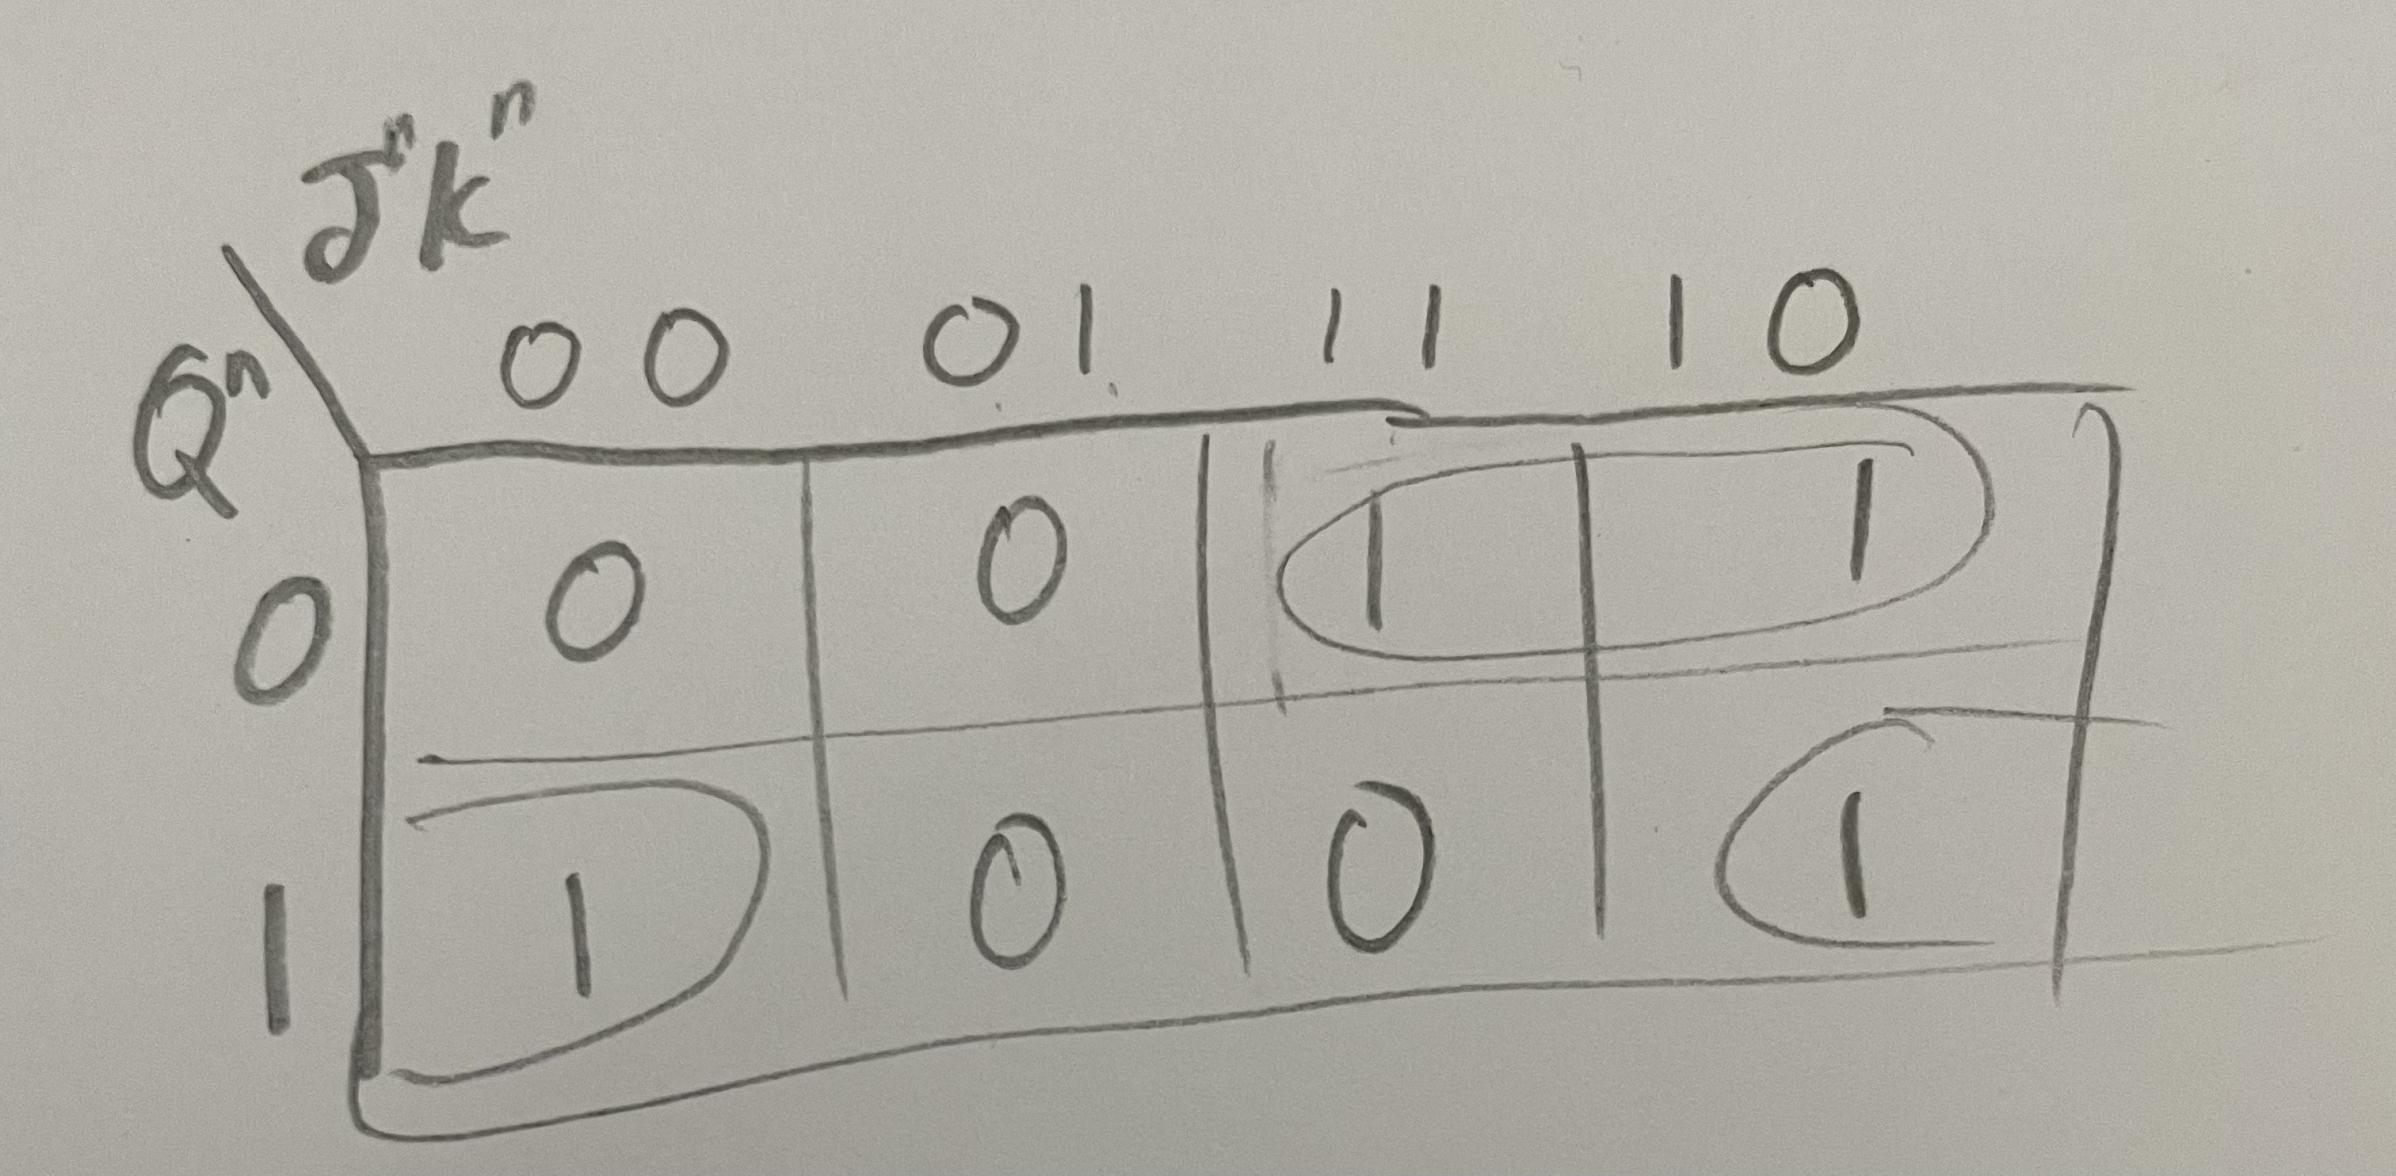
\includegraphics[scale=0.15]{Problem1.jpg}
$$Q^{n+1}=J^{n}.\overline{Q^n}+\overline{K^n}.Q^n$$
\subsection*{(d)}
The transition table of  the D latch is:
\begin{center}
    \begin{tabular}{|c|c||c|}
        C & D & Q next \\
        \hline
        0 & x & Q \\
        \hline
        1 & 0 & 0 \\
        \hline
        1 & 1 & 1 \\
        \hline
    \end{tabular}
\end{center}
Which is the same as the transition table of the JK latch with $J=\bar{K}=D$.
\begin{center}
    \begin{tabular}{|c|c|c||c|}
        C & J=D & $K=\bar{D}$ & Q next \\
        \hline
        0 & x & x & Q \\
        \hline
        1 & 0 & 1& 0 \\
        \hline
        1 & 1 & 0 & 1 \\
        \hline
    \end{tabular}
\end{center}
\end{document}